\documentclass{minimal}
\usepackage{pgfplots}
\usepackage[european,straightvoltages]{circuitikz}
\pgfplotsset{compat=1.16}

\begin{document}

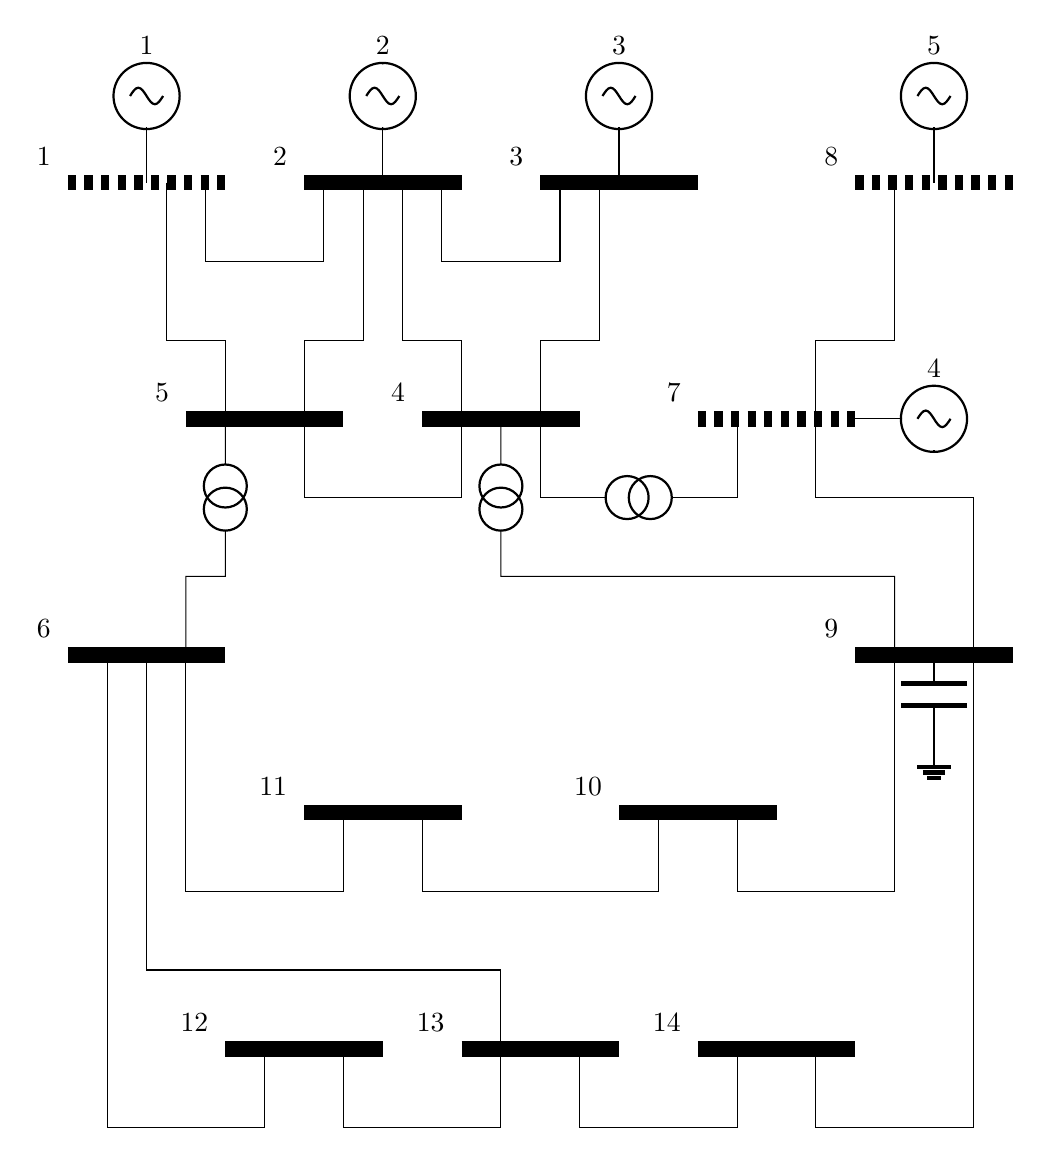
\begin{tikzpicture}[scale=1,transform shape]
    %	\draw [lightgray,ultra thin] (0,0) grid(13,16);
    % % ----- nodes ----- % %
    \draw [line width = 2mm,dashed] (1,14) node[anchor = south east] {1} -- ++(2,0); 	% Bus 1
    \draw [line width = 2mm] (4,14) node[anchor = south east] {2} -- ++(2,0); 	% Bus 2
    \draw [line width = 2mm] (7,14) node[anchor = south east] {3} -- ++(2,0); 	% Bus 3
    \draw [line width = 2mm,dashed] (11,14) node[anchor = south east] {8} -- ++(2,0); 	% Bus 8
    \draw [line width = 2mm] (2.5,11) node[anchor = south east] {5} -- ++(2,0); 	% Bus 5
    \draw [line width = 2mm] (5.5,11) node[anchor = south east] {4} -- ++(2,0); 	% Bus 4
    \draw [line width = 2mm,dashed] (9,11) node[anchor = south east] {7} -- ++(2,0); 	% Bus 7
    \draw [line width = 2mm] (1,8) node[anchor = south east] {6} -- ++(2,0); 		% Bus 6
    \draw [line width = 2mm] (11,8) node[anchor = south east] {9} -- ++(2,0); 	% Bus 9
    \draw [line width = 2mm] (4,6) node[anchor = south east] {11} -- ++(2,0); 		% Bus 11
    \draw [line width = 2mm] (8,6) node[anchor = south east] {10} -- ++(2,0); 		% Bus 10
    \draw [line width = 2mm] (3,3) node[anchor = south east] {12} -- ++(2,0); 		% Bus 12
    \draw [line width = 2mm] (6,3) node[anchor = south east] {13} -- ++(2,0); 		% Bus 13
    \draw [line width = 2mm] (9,3)node[anchor = south east] {14}  -- ++(2,0); 		% Bus 14
    % % ----- lines ----- % %
    \draw (2.75,14) -- ++(0,-1) -- ++(1.5,0) -- ++(0,1); 		% 1-2
    \draw (5.75,14) -- ++(0,-1) -- ++(1.5,0) -- ++(0,1); 		% 2-3
    \draw (2.25,14) -- ++ (0, -2) -- ++(0.75,0) -- ++ (0,-1); 	% 1-5
    \draw (4.75,14) -- ++(0,-2) -- ++(-0.75,0) -- ++(0,-1); 	% 2-5
    \draw (5.25,14) -- ++(0,-2) -- ++(0.75,0) -- ++(0,-1); 		% 2-4
    \draw (7.75,14) -- ++(0,-2) -- ++(-0.75,0) -- ++(0,-1); 	% 3-4
    \draw (4,11) -- ++(0,-1) -- ++(2,0) -- ++(0,1); 			% 5-4
    \draw (7,11) -- ++(0,-1) to[voosource] ++(2.5,0) -- ++(0,1); 			% 4-7
    \draw (10.5,11) -- ++(0,1) -- ++(1,0) -- ++(0,2);			% 7-8
    \draw (10.5,11) -- ++(0,-1) -- ++(2,0) -- ++(0,-2); 		% 7-9
    \draw (6.5,11) to[voosource] ++(0,-2) -- ++(5,0) -- ++(0,-1);			% 4-9
    \draw (3,11) to[voosource] ++(0,-2) -- ++(-0.5,0) -- ++(0,-1);			% 5-6
    \draw (2.5,8) -- ++(0,-3) -- ++(2,0) -- ++(0,1);			% 6-11
    \draw (1.5,8) -- ++(0,-6) -- ++(2,0) -- ++(0,1);			% 6-12
    \draw (2,8) -- ++(0,-4) -- ++(4.5,0) -- ++(0,-1);			% 6-13
    \draw (5.5,6) -- ++(0,-1) -- ++(3,0) -- ++(0,1);			% 11-10
    \draw (9.5,6) -- ++(0,-1) -- ++(2,0) -- ++(0,3);			% 10-9
    \draw (4.5,3) -- ++(0,-1) -- ++(2,0) -- ++(0,1);			% 12-13
    \draw (7.5,3) -- ++(0,-1) -- ++(2,0) -- ++(0,1);			% 13-14
    \draw (10.5,3) -- ++(0,-1) -- ++(2,0) -- ++(0,6);			% 14-9
    % % ----- gens ----- % %
    \draw [] (2,15.5) node[above]{1} to[sinusoidal voltage source] ++(0,-0.8);
    \draw [] (5,15.5) node[above]{2} to[sinusoidal voltage source] ++(0,-0.8);
    \draw [] (8,15.5) node[above]{3} to[sinusoidal voltage source] ++(0,-0.8);
    \draw [] (12,15.5) node[above]{5} to[sinusoidal voltage source] ++(0,-0.8);
    \draw [] (12,11.4) node[above]{4} to[sinusoidal voltage source] ++(0,-0.8);
    % % ----- gen-lines ----- % %
    \draw (2,14.7) -- ++(0,-0.7);
    \draw (5,14.7) -- ++(0,-0.7);
    \draw (8,14.7) -- ++(0,-0.7);
    \draw (12,14.7) -- ++(0,-0.7);
    \draw (11.6,11) -- ++(-0.7,0);
    % % ----- shunt susc ----- % %
    %\draw (12,7) node[ground]{}(G);
    \draw [thick] (12,8) to[C] ++(0,-1) node[ground]{};
    \end{tikzpicture}
\end{document}

% !TEX program = pdflatex
